\documentclass[]{elsarticle} %review=doublespace preprint=single 5p=2 column
%%% Begin My package additions %%%%%%%%%%%%%%%%%%%
\usepackage[hyphens]{url}
\usepackage{lineno} % add
\providecommand{\tightlist}{%
  \setlength{\itemsep}{0pt}\setlength{\parskip}{0pt}}

\bibliographystyle{elsarticle-harv}
\biboptions{sort&compress} % For natbib
\usepackage{graphicx}
\usepackage{booktabs} % book-quality tables
%% Redefines the elsarticle footer
%\makeatletter
%\def\ps@pprintTitle{%
% \let\@oddhead\@empty
% \let\@evenhead\@empty
% \def\@oddfoot{\it \hfill\today}%
% \let\@evenfoot\@oddfoot}
%\makeatother

% A modified page layout
\textwidth 6.75in
\oddsidemargin -0.15in
\evensidemargin -0.15in
\textheight 9in
\topmargin -0.5in
%%%%%%%%%%%%%%%% end my additions to header

\usepackage[T1]{fontenc}
\usepackage{lmodern}
\usepackage{amssymb,amsmath}
\usepackage{ifxetex,ifluatex}
\usepackage{fixltx2e} % provides \textsubscript
% use upquote if available, for straight quotes in verbatim environments
\IfFileExists{upquote.sty}{\usepackage{upquote}}{}
\ifnum 0\ifxetex 1\fi\ifluatex 1\fi=0 % if pdftex
  \usepackage[utf8]{inputenc}
\else % if luatex or xelatex
  \usepackage{fontspec}
  \ifxetex
    \usepackage{xltxtra,xunicode}
  \fi
  \defaultfontfeatures{Mapping=tex-text,Scale=MatchLowercase}
  \newcommand{\euro}{€}
\fi
% use microtype if available
\IfFileExists{microtype.sty}{\usepackage{microtype}}{}
\ifxetex
  \usepackage[setpagesize=false, % page size defined by xetex
              unicode=false, % unicode breaks when used with xetex
              xetex]{hyperref}
\else
  \usepackage[unicode=true]{hyperref}
\fi
\hypersetup{breaklinks=true,
            bookmarks=true,
            pdfauthor={},
            pdftitle={Foreign direct investment, corporate social responsibility, and malaria control in Mozambique - trends, risks, and opportunities},
            colorlinks=true,
            urlcolor=blue,
            linkcolor=magenta,
            pdfborder={0 0 0}}
\urlstyle{same}  % don't use monospace font for urls
\setlength{\parindent}{0pt}
\setlength{\parskip}{6pt plus 2pt minus 1pt}
\setlength{\emergencystretch}{3em}  % prevent overfull lines
\setcounter{secnumdepth}{0}
\usepackage{longtable}
% Pandoc toggle for numbering sections (defaults to be off)
\setcounter{secnumdepth}{0}
% Pandoc header
\usepackage{longtable}


\usepackage[nomarkers]{endfloat}

\begin{document}
\begin{frontmatter}

  \title{Foreign direct investment, corporate social responsibility, and malaria
control in Mozambique - trends, risks, and opportunities}
    \author[isglobal,cism,vu]{Joe Brew\corref{c1}}
   \ead{joebrew@economicsofmalaria.com} 
   \cortext[c1]{Corresponding Author}
    \author[isglobal,icl,cism]{Elisa Sicuri}
   \ead{elisa.sicuri@isglobal.org} 
  
      \address[isglobal]{Barcelona Institute for Global Health, c/ Rosselló, 132, 5è 2a. 08036,
Barcelona, Spain}
    \address[icl]{Imperial College London, South Kensington Campus, London SW7 2AZ, U.K.}
    \address[cism]{Centro de Investigação em Saúde de Manhiça, Vila da Manhiça, Bairro
Cambeve, Rua 12, Distrito da Manhiça, CP 1929, Maputo, Mozambique}
    \address[vu]{VU University Amsterdam, De Boelelaan 1105, 1081 HV Amsterdam,
Netherlands}
  
  \begin{abstract}
  Foreign direct investment (FDI) in Mozambique has increased rapidly in
  the last two decades. The growing interest in corporate social
  responsibility (CSR) - combined with a recent push for malaria
  elimination - suggest the need for a critical examination of the role of
  FDI in malaria control and elimination. Through a systematic review of
  the literature, we find that there has been a notable increase in
  research pertaining to FDI, CSR and malaria in recent years. Consensus
  among researchers is that this increase has not been accompanied by a
  substantial private sector investment in malaria control (with a few
  notable exceptions). This suggests a potential opportunity for scaling
  up privately driven malaria control as a means to both improve public
  health and increase return on investment. However, given the lack of
  coordination between public and private sectors, even when interests
  coincide, an over-reliance on foreign and private initiative for funding
  eradication is not without risks.
  \end{abstract}
  
 \end{frontmatter}

\subsection{Abstract}\label{abstract}

Foreign direct investment (FDI) in Mozambique has increased rapidly in
the last two decades. The growing interest in corporate social
responsibility (CSR) - combined with a recent push for malaria
elimination - suggest the need for a critical examination of the role of
FDI in malaria control and elimination. Through a systematic review of
the literature, we find that there has been a notable increase in
research pertaining to FDI, CSR and malaria in recent years. Consensus
among researchers is that this increase has not been accompanied by a
substantial private sector investment in malaria control (with a few
notable exceptions). This suggests a potential opportunity for scaling
up privately driven malaria control as a means to both improve public
health and increase return on investment. However, given the lack of
coordination between public and private sectors, even when interests
coincide, an over-reliance on foreign and private initiative for funding
eradication is not without risks.

\subsection{Introduction}\label{introduction}

Mozabique's recent economic growth has been facilitated by the
government's open policy towards foreign investment, a plentiful supply
of natural resources (particularly minerals and hydrocarbons) (Rogers
2014) and relatively inexpensive labor. Improvements in health have
accompanied economic expansion, but Mozambique still lags behind in
basic health outcomes - particularly those related to malaria - even by
regional standards. Most economic activities have to deal with malaria:
particularly agricultural-based and extraction activities cannot be
carried out without consistent investment towards malaria management,
both prevention and prompt treatment. This can be done as part of the
``normal activities'' of private sector or can go slightly beyond what
is strictly needed for the activities and be seen as part of the
corporate social responsibilityDespite strong evidence showing that
improved health yields substantial economic benefits (Brundtland 1999,
Bloom and Canning (2008)), there is little evidence regarding the extent
to which ``corporate social responsibility'' (CSR) activities of foreign
firms have targeted or impacted malaria. Understanding the relationship
between FDI, CSR and malaria is essential to identifying which
incentives and barriers to private sector involvement in malaria
elimination exist, as well as identifying potential opportunities and
synergies for scaling up private sector involvment in malaria
elimination.

That said, The few malaria-related CSR projects in recent years has come
in large, ``mega-projects'' whose well-publicized malaria abatement
activities are profit-driven (Mouzin and al. 2011) or whose primary aim
is not profit-related (Han 2015). Though the former is often portrayed
as a ``win-win'' for business and public health, the latter also offers
tangible benefits for private industry, and should be understood as
operating under the same conditions and with the same motivations.

Private foreign investors showed a great optimism during the FMI meeting
held in Maputo in 2014 (reference needed). Beginning in late 2015, the
flood of FDI into Mozambique (and many other subsaharan African nations)
slowed to a trickle. The impact of this slowdown on CSR is not yet
known, but it can reasonably be assumed that it will mean a reduction in
CSR activities (albeit with lag). Almost in parallel to this, Mozambique
has had serious financial problems which have resulted in default
(reference needed
http://www.economist.com/news/middleeast-and-africa/21715030-mozambique-fails-pay-its-debtsmozambiques-default).
Given the rapidly changing economic and epidemiologic context in
Mozambique, a comprehensive and current understanding of both (a) the
landscape of FDI and CSR in Mozambique and (b) public health issues
(namely, malaria control) which are directly affected those investments
is sorely needed. Such an understanding may foster greater private
interest in for-profit investment in public health measures. Likewise,
it can facilitate better public sector understanding of potential
industry partners and stakeholders (a prerequisite to greater
public-private collaborations), and guide the public sector away from an
inflexible dependence on FDI for the provision of public health
necessities.

We carried out a systematic review of economic and public health
research pertaining to FDI, CSR, malaria and Mozambique. This paper
gives an overview of trends in FDI and CSR in Mozambique as well as a
synthesis of academic literature on the topic, with a focus on its
impact on malaria control. It is by no means comprehensive, but offers a
consolidated starting point for understanding both the place of FDI and
CSR in the literature, as well as where the interests and incentives of
the public and private sectors converge and differ in regards to malaria
control.

\section{Methods}\label{methods}

We sought to identify and describe sources of information regarding FDI
and CSR in Mozambique, particularly in regards to malaria control and
elimination. We carried out this identification process via 2 distinct
approaches to understanding FDI, CSR and malaria in Mozambique:

\begin{enumerate}
\def\labelenumi{\arabic{enumi}.}
\tightlist
\item
  Identification and analysis of quantitative datasets.
\item
  Systematic review of both grey literature (news, company websites,
  etc.) and academic literature.
\end{enumerate}

\subsection{Quantitative datasets}\label{quantitative-datasets}

We examined and analyzed trends from multiple datasets related to FDI,
CSR and malaria in Mozambique. These included the ``Doing Business''
data pertaining to the measurement of regulatory efficiency, the GADM,
the Deutsche Bundesbank Data Repository for foreign exchange rate
history, the Knoema World Data Atlas for macroeconomic trends, the World
Bank data portal for information containing to net foreign inflows and
FDI, USAID Demographic and Health Survey data on sociodemographics and
health-related practices, the Instituto Nacional de Estatistica for
granular data pertaining to Mozambique's population and economic
activities, and Institute for Health Metrics and Evaluation data
pertaining to disease trends over time.

\subsection{Systematic review}\label{systematic-review}

\subsubsection{Grey literature}\label{grey-literature}

Our grey literature review followed known practices (Godin et al. 2015,
Adams et al. (2016)), relying on internet searches and linked
references. Sources include, but are not limited to UN reports on
economic trends, WHO reports and brochures pertaining to health trends,
company websites and brochures, newspaper articles, and think-tank white
papers.

\subsubsection{Academic literature}\label{academic-literature}

In order to gauge research attention and focus on FDI and CSR insofar as
they affect Mozambique and malaria, four systematic searches were
carried out using the EBSCOhost and NCBI/pubmed databases. Our search
queries are detailed below:

\begin{enumerate}
\def\labelenumi{\arabic{enumi}.}
\tightlist
\item
  \texttt{"(malaria)\ and\ (corporate\ social\ responsibility)"} (no
  results found in EBSCO)
\item
  \texttt{"(malaria)\ and\ (foreign\ direct\ investment)"}
\item
  \texttt{"(mozambique)\ and\ (corporate\ social\ responsibility)"} (no
  resuts found in EBSCO)
\item
  \texttt{"(mozambique)\ and\ (foreign\ direct\ investment)"}
\end{enumerate}

\section{Results}\label{results}

\subsection{Quantitiative datasets pertaining to FDI and CSR in
Mozambique}\label{quantitiative-datasets-pertaining-to-fdi-and-csr-in-mozambique}

\subsubsection{Sources of FDI in
Mozambique}\label{sources-of-fdi-in-mozambique}

According to the IMF, 69 countries had foreign direct investment in
Mozambique as of the end of 2015. The below chart shows the top 10
countries ranked by amount invested in Mozambique.

\begin{center}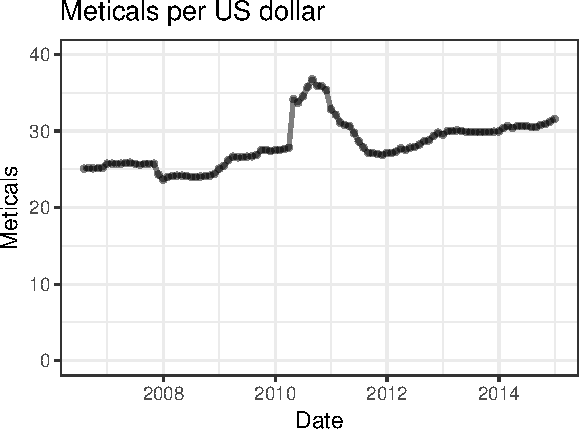
\includegraphics{paper_files/figure-latex/unnamed-chunk-6-1} \end{center}

What stands out is the presence of many ``non-Western'' countries in the
top 10. Though data are not available over time (ie, we cannot make
temporal comparisons), the landscape of investment 20 years prior would
have been both (a) far smaller and (b) primarily composed of western
countries.

\subsubsection{Massive increase in FDI}\label{massive-increase-in-fdi}

Following independence (1974), Mozambique saw two decades of low and
unsteady foreign investment, largely due to the civil war (which did not
end until 1992). Thereafter, foreign investment began a steady increase
but leveled off by the late 1990s. However, the discovery of novel
sources of oil and gas set off a new spur of investments beginning in
2007, and continuing through last year. From 2010 to 2013, foreign
direct investment grew from 1.26 to 6.70 billion USD, a more than
five-fold increase (WB 2015).

\begin{center}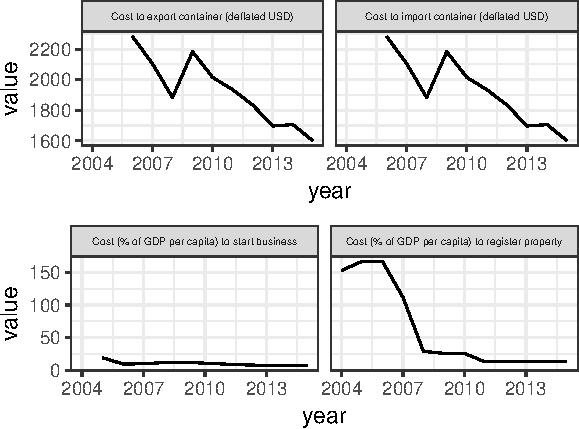
\includegraphics{paper_files/figure-latex/unnamed-chunk-7-1} \end{center}

In addition to the discovery of new resources, recent growth has also
been fueled by political and economic reforms which have made it easier
for foreigners to do business in Mozambique. Of particular note,
inflation remained relatively low (at least through 2014) (Bundesbank
2015).

\begin{center}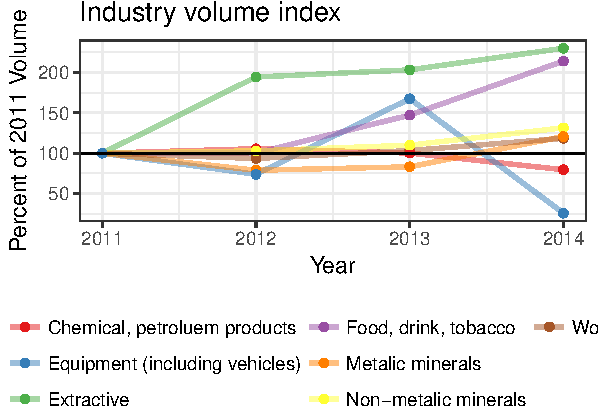
\includegraphics{paper_files/figure-latex/unnamed-chunk-8-1} \end{center}

The massive increases in FDI have also been facilitated by dramatic
decreases in the costs to import and export, as well as the costs of
starting a business and registering property (Bank 2016).

\begin{center}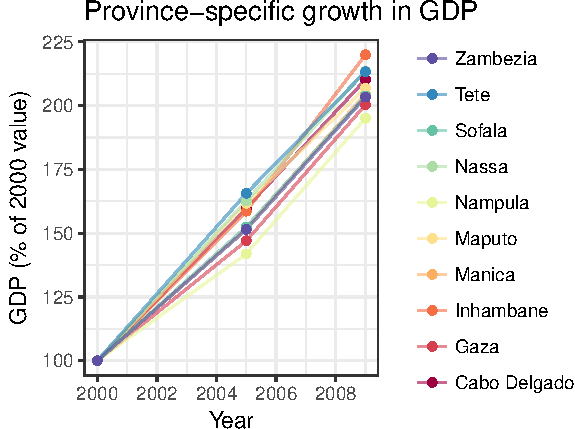
\includegraphics{paper_files/figure-latex/unnamed-chunk-9-1} \end{center}

\subsubsection{Breakdown by industry}\label{breakdown-by-industry}

Most of recent growth has come in the ``extractive'' industries, a term
encompassing a range of industry, but in the Mozambican context largely
applying to hydrocarbons and mining (INE 2015).

\begin{center}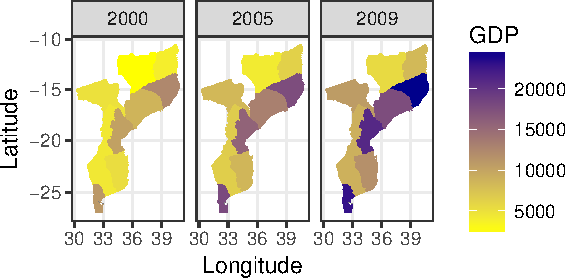
\includegraphics{paper_files/figure-latex/unnamed-chunk-10-1} \end{center}

The late 2015 economic slow-down in the developing world, particularly
the low price of oil, could have serious repercussions for FDI in
Mozambique. That said, the mining of metals and the service industries
both make up a larger share of Mozambique's economic output than the
extraction of hydrocarbons, which should somewhat buffer the Mozambican
economy from the negative effects of low oil prices.

\subsubsection{Breakdown by region}\label{breakdown-by-region}

Despite the concentration of private investment in regional projects,
growth has been similarly large in all provinces From 2000 to 2009, GDP
approximately doubled, with the greatest growth occurring in Inhambane
(119\% growth from 2000 to 2009), and the least robust grwoth in Nampula
(95\%) (Knoema 2015).

\begin{center}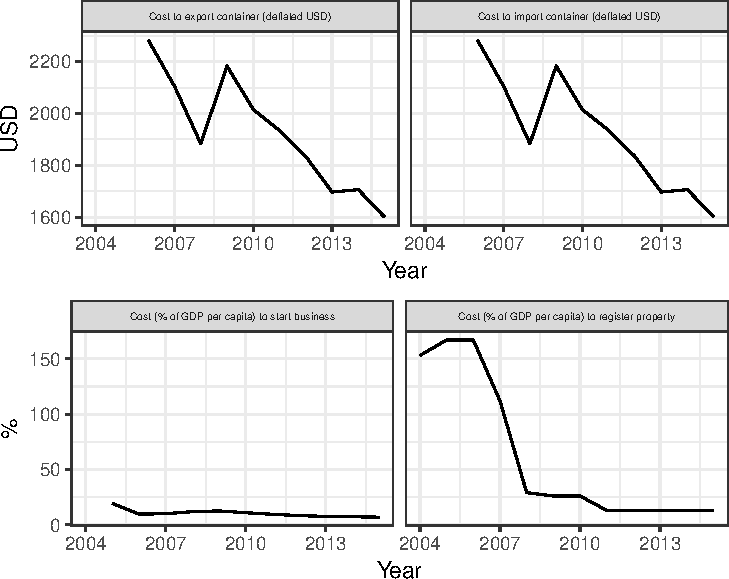
\includegraphics{paper_files/figure-latex/unnamed-chunk-11-1} \end{center}

The homogeneity in growth comes somewhat as a surprise, as it defies the
general developing world pattern in that growth in areas that already
had high GDP (Maputo and the coastal provinces) was as robust as growth
in areas with previously low GDP.

\begin{center}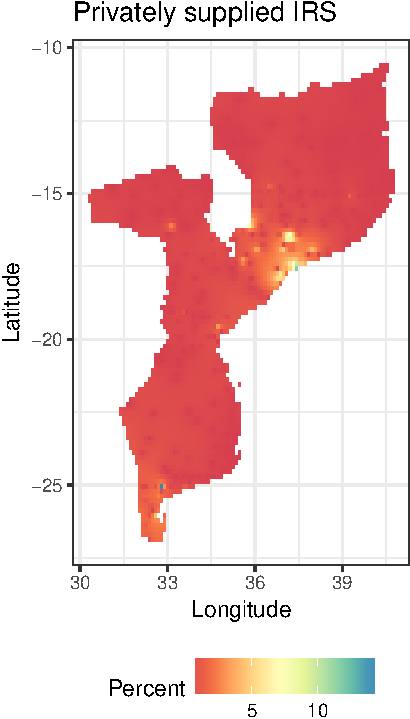
\includegraphics{paper_files/figure-latex/unnamed-chunk-12-1} \end{center}

\subsubsection{CSR in Mozambique}\label{csr-in-mozambique}

Corporate social responsibility in Mozambique is new in nomenclature,
but activities which could be classified as CSR have existed for
decades. The number of firms actively engaging in CSR cannot be
ascertained (given the large and ever-changing number of small
businesses), but virtually all of the largest firms, both foreign and
domestic, have a CSR component.

Firms with CSR activities are often large and foreign. Among the largest
``key players'' in Mozambican CSR are Coca-Cola, British Petroleum and
Colgate-Palmolive. State conglomerates, such as Águas de Moçambique and
Electricidade de Moçambique, also participate in CSR activities (Compact
2007).

\subsubsection{Malaria-related CSR and other corporate
activity}\label{malaria-related-csr-and-other-corporate-activity}

Most CSR-funded activities are focused on education, community
development, women's rights and entrepreneurship. According to a UN
poll, none of the country's largest firms invest directly in
malaria-related CSR activities (Compact 2007). This may be due to the
perceived costs of malaria control, lack of perceived PR benefits, the
government and NGO's predominant role in the area, as well as the
``opt-in'' nature and privacy/legal issues generally related to engaging
in health-related campaigns.

That said, a majority of the firms interviewed by the UN indicated that
one of the principal reasons for investment in CSR is to complement
government efforts. To the extent that malaria accounts for more of the
loss in disability-adjusted life years in Mozambique than comparable
countries (IHME 2015), malaria control's lack of representation among
core CSR activities is a notable absence.

Whether under the guise of CSR or not, it is noteworthy that the private
sector currently does play a role in malaria control activities.
According to 2011 DHS data, greater than 7 in every 1,000 households had
a private company carry out indoor residual spraying (DHS 2011). And, in
some clusters, the percent of houses covered by private IRS was greater
than 25\%.

Interestingly, though the UN data indicated that corporations don't
actively engage in malaria control as part of CSR, the geographic
distribution of households which had their homes sprayed by a private
entity are clustered in areas where foreign firms operate, particularly
in the south (around Maputo) in the East, where extractive industry
activity is highest.

\begin{center}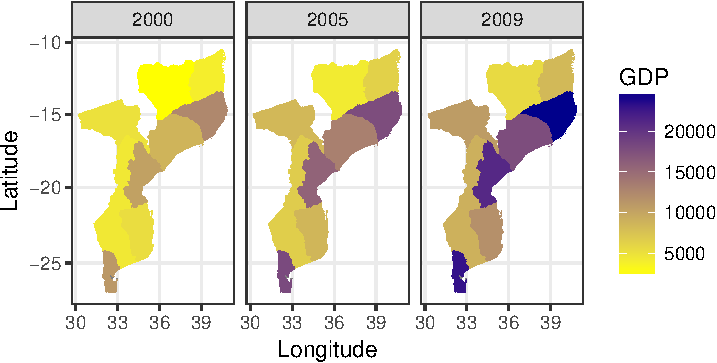
\includegraphics{paper_files/figure-latex/unnamed-chunk-14-1} \end{center}

\subsection{Systematic review}\label{systematic-review-1}

\subsubsection{Grey literature}\label{grey-literature-1}

\paragraph{Grey literature search
strategy}\label{grey-literature-search-strategy}

We devised 2 simple search queries, and use www.google.com and
www.bing.com to retrieve results. The queries were:

\begin{enumerate}
\def\labelenumi{\arabic{enumi}.}
\tightlist
\item
  \texttt{Mozambique\ foreign\ direct\ investment\ malaria}
\item
  \texttt{Mozambique\ corporate\ social\ responsibility\ malaria}
\end{enumerate}

\paragraph{Grey literature search
results}\label{grey-literature-search-results}

Google returned 266,000 results for the former query, and 240,000 for
the latter (506,000 in total); Bing returned 4,620 and 20,900,
respectively. We screened the top 50 results from both services (a total
of 100 items) for both queries For the former, of the 100 items
identified, 33 were identical in both search engines (yielding a total
of 67 unique items); in the latter, 39 were identical (yielding a total
of 61 unique items).

\begin{center}
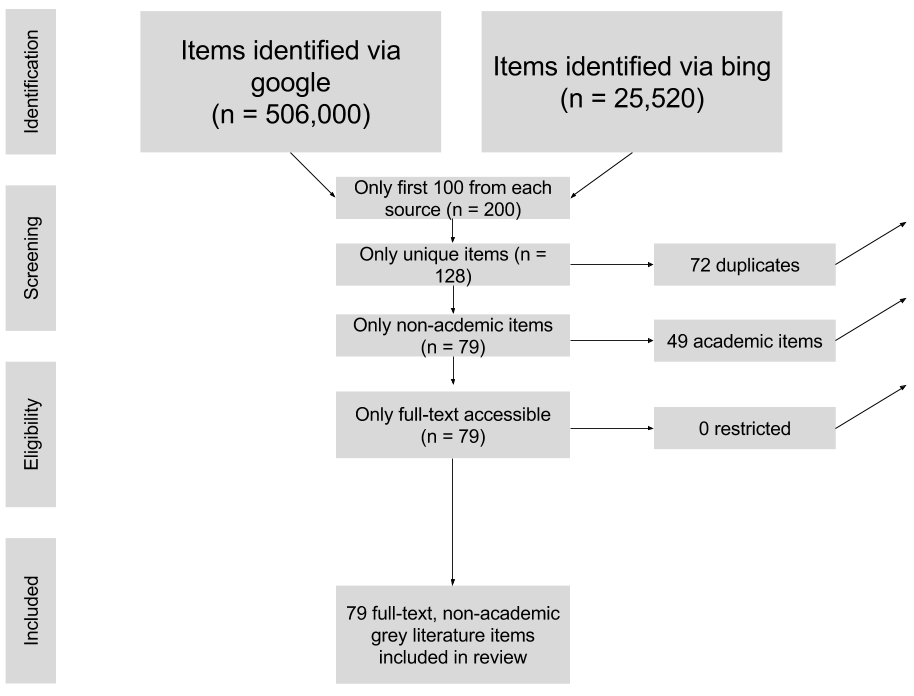
\includegraphics[width=400pt]{img/prisma_grey.png}
\end{center}

\paragraph{Grey literature synthesis}\label{grey-literature-synthesis}

Our grey literature review returned relatively little information which
was not readily available in those sources uncovered in the data review
and systematic review. Very few foreign companies operating in
Mozambique have any publicly available information regarding corporate
social responsibility activities.

One notable exception is the Nando's-lead Goodbye Malaria Trust, an
umbrella organization which inclues a development impact bond, the
Goodbye Malaria initiative, and partnerships with several other foreign
firms operating in Mozambique (more details here).

\subsubsection{Academic literature}\label{academic-literature-1}

Our search is outlined in the below PRISMA-based diagram.

\begin{center}
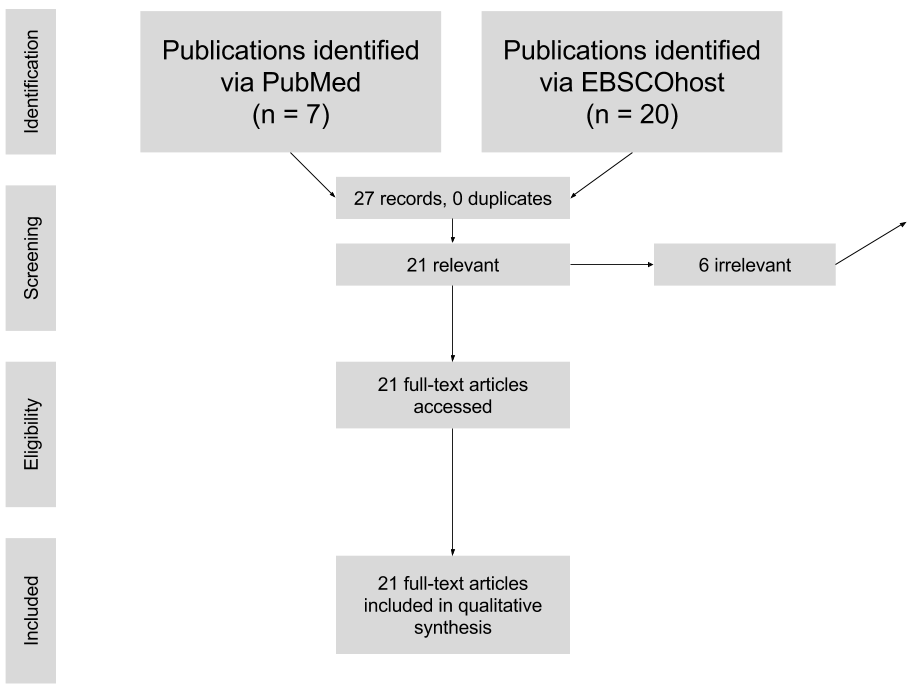
\includegraphics[width=400pt]{img/prisma.png}
\end{center}

The below table shows the results retrieved for the systematic review.
Full article information is in the bibliography

\begingroup\fontsize{6pt}{7pt}\selectfont

\begin{longtable}{lllll}
  \hline
Source & Year & Title & Type & Author \\ 
  \hline
EBSCOhost & 2009 & Public Governance, H... & FDI Malaria & Azemar, et al \\ 
  EBSCOhost & 2014 & A Critical Review of... & FDI MOZ & Mahembe, et al \\ 
  EBSCOhost & 2000 & Administrative barri... & FDI MOZ & Emery, et al \\ 
  EBSCOhost & 2012 & Attracting Foreign D... & FDI MOZ & Tembe, et al \\ 
  EBSCOhost & 2013 & Contemporary Process... & FDI MOZ & German, et al \\ 
  EBSCOhost & 2012 & Corruption and Multi... & FDI MOZ & Grande, et al \\ 
  EBSCOhost & 2014 & Determining the Natu... & FDI MOZ & Winkler, et al \\ 
  EBSCOhost & 1999 & Foreign Direct Inves... & FDI MOZ & Morisset, et al \\ 
  EBSCOhost & 2002 & Foreign Direct Inves... & FDI MOZ & Bassu, et al \\ 
  EBSCOhost & 2014 & Growth, Capital Accu... & FDI MOZ & Castel-Branco, et al \\ 
  EBSCOhost & 2007 & Linkage Between fore... & FDI MOZ & Wilson, et al \\ 
  EBSCOhost & 2012 & Mining FDI and Infra... & FDI MOZ & Robbins, et al \\ 
  EBSCOhost & 2013 & Potential and actual... & FDI MOZ & Winkler, et al \\ 
  EBSCOhost & 2004 & Regional integration... & FDI MOZ & Goldstein, et al \\ 
  EBSCOhost & 2014 & Sector Case Study: M... & FDI MOZ & Barnard, et al \\ 
  EBSCOhost & 2011 & Strategic Privatisat... & FDI MOZ & Buur, et al \\ 
  EBSCOhost & 2016 & The Economics and Po... & FDI MOZ & Hansen, et al \\ 
  EBSCOhost & 2002 & The Role of FDI in E... & FDI MOZ & Bjorvatn, et al \\ 
  EBSCOhost & 2010 & Uncovering Trends in... & FDI MOZ & Warren-Rodriguez, et al \\ 
  EBSCOhost & 2014 & Sector Case Study: A... & FDI MOZ & Barnard, et al \\ 
  Pubmed & 2004 & Community health out... & CSR & Singer, et al \\ 
  Pubmed & 2014 & Public-private partn... & CSR & Hutton, et al \\ 
  Pubmed & 2007 & Feasibility of water... & CSR MOZ & Tang, et al \\ 
  Pubmed & 2002 & The economic impact ... & FDI & Mills, et al \\ 
  Pubmed & 2004 & The economic burden ... & FDI & Russell, et al \\ 
  Pubmed & 2012 & The economic benefit... & FDI & Feachem, et al \\ 
  Pubmed & 2012 & Global health fundin... & FDI & D'Agostino, et al \\ 
  Pubmed & 2015 & Tracking Global Fund... & FDI & Huntington, et al \\ 
   \hline
\hline
\end{longtable}

\endgroup

The below chart shows our systematically retried publications by date.
What is most striking is how little academic attention has been given to
CSR, with none given to the intersection of CSR and malaria.

\begin{center}\includegraphics{paper_files/figure-latex/unnamed-chunk-17-1} \end{center}

\subsubsection{Qualitative synthesis of systematic review of academic
literature}\label{qualitative-synthesis-of-systematic-review-of-academic-literature}

The literature is largely clear on two points: (1) that economic growth
in Mozambique has been fueled in large part by foreign direct
investment, and (2) that economic growth has been accompanied by a rapid
decrease in malaria morbidity and mortality. There is no clear consensus
regarding the extent to which the former is a result of the latter, and
researchers disagree on how much of a role FDI has played in improving
the social and economic conditions of Mozambicans.

Mozambique has a unique social and economic system, which is
particularly attractive to foreign investment. The Mozambican economy is
``oriented to incentivize large-scale FDI projects'' (Robbins and
Perkins 2012). Land distribution, for example, despite being
igualitarian \emph{de juro} has been \emph{de facto} aimed at satisfying
the interests of large foreign firms (German, Schoneveld, and Mwangi
2013). In extractive industries, and particular the sugar industry, the
state has gone so far as to encourage unprofitable entreprise by
propping up an internal market so as to keep foreign inflows of cash
from drying out, a process described as a ``mediating bureaucracy''
(Buur, Tembe, and Baloi 2012). Another part of the attraction of FDI to
Mozambique is the extent to which the state and society, both formally
and informally, subsidize the cost of labor by allowing for below
subsistence wages.

In one view, the last two decades of economic growth are largely
irrelevant to the well-being of Mozambicans due to the ``porous and
extractive'' nature of FDI (Castel-Branco 2014). In other words, since
both investment and profit are largely external to the Mozambican
economy and society, ``positive spillovers'' into local firms are few
and far between (Winkler 2013).

CSR is one way of offsetting the trend, and its potential for mutually
beneficial effects is high, particularly when its resources target
malaria control. Per one analysis, malaria elimination in an endemic
country like Mozambique would lead to a 16\% increase in FDI (Azemar and
Desbordes 2009). The possibility of re-directing resource rents to
socially beneficial ends is acknolwedged by multiple authors (Robbins
and Perkins 2012, Castel-Branco (2014)).

However, the re-direction or resource rents to CSR is complicated. If
coerced (through higher taxes or fewer incentives to investment), the
recent decrease in FDI may be exacerbated. If voluntary, particularly in
the case of expenditures in medicine and health, the public's health
would be largely dependent on private whim, a recipe for
unsustainability at best and potential epidemiologic catastrophe at
worst.

In summary, Mozambique's high ratio of FDI to GDP and general allowance
of ``porous'' foreign investment represents an opportunity for scaling
up the private sector's engagement with public health, as a means to
offset the lack of social benefits that traditional FDI has entailed. A
coercive (tax-based) approach to scaling up this engagement may lead to
a withdrawl of FDI from the country. The alternative, an increase in
CSR, is a possible route for creating synergies, particular in the case
of malaria elimination.

\section{Discussion}\label{discussion}

\subsection{Scaling up malaria control through CSR: opportunity and
risk}\label{scaling-up-malaria-control-through-csr-opportunity-and-risk}

\subsubsection{Opportunity}\label{opportunity}

The historical absence of malaria-related CSR represents an opportunity
for complementarity. In addition to improvements in public health, both
the private and public sectors stand to benefit economically from a
scaling up of malaria control driven by the private sector. By
increasing malaria control activities, as a share of total CSR
expenditures, public funds could be redirected towards other areas of
health. Likewise, if private CSR activities pivoted towards malaria
control rather more general philanthropical gestures, CSR would have a
more direct impact on wellbeing (with less temporal lag), thereby
fulfilling the public relations goals of the firms that invest in CSR.
Finally, for many industries, the firm itself is a potential direct
beneficiary, given that improvements in employee health and a reduction
in employee absenteeism can be directly correlated to productivity.

\subsubsection{Risk}\label{risk}

Scaling up CSR while also encouraging its redirection towards malaria
control is not without risks. The most notable downfall of this approach
is the potential for the inadvertent dependence on the private sector
for what is essentially a public good. Were CSR targeting malaria
control to reach significant levels (and the government were to enact a
correspoding redirection of funds towards the financing of other health
areas), then a situation would be created in which the public sector had
essentially divested from a public good. This would be unwise and
dangerous.

A secondary risk is that increased private sector involvement in malaria
control could cause a decrease in public sector \emph{competence} in the
prevention and treatment of malaria. This could have negative
consequences in the case of either a financial or economic crisis (in
which CSR activity would be curtailed) or an increase in malarial
activity. By the same token, CSR involvement in malaria control could
potentially portend, at least initially, less effective interventions.
Private firms' incentives, though aligned with the public's in terms of
malaria, are not identical, and pressures from shareholders and for
positive public perception might motivate malaria control strategies
which do not necessarily carry with them the most recent scientific
knowledge.

A third risk is a lack of coordination. Both in terms of logistical
activities as well as biological realities (drug and insecticide
resistance, etc.), coordination of malaria control activities is
absolutely essentially if Mozambique is going to make the transition to
eradication. The issue of coordination could be solved through an
activities and outcomes reporting/surveillance structure (necessarily
managed by the state), but compliance could be problematic.

A final risk is that of volatility. By centralizing malaria control
under the auspices of the government, public health authorities can
effectively distribute malaria control expenditures to where and when
they are most needed. If this control were only in the hands of private
firms, expenditure would likely transform into a function of
firm-specific profitability and shareholder incentives, as well as
market cycles. This could lead to a situation in which malaria control
activities are most prevalent in areas where the economy is strongest,
rather than areas where the need is greatest.

\section{Conclusion}\label{conclusion}

High FDI in Mozambique and growing interest in CSR both call for
increased reflection on the private sector's role in the delivery of
public goods. A refocusing of CSR expenditures into areas where the need
is greatest (specifically, malaria control) could lead to better health
and greater profits. This ``win-win'' for the public and private sectors
represents a rare opportunity, which deserves more discourse, research
and experimentation.

That said, the growing interest in CSR suggests both that (a) the need
for services exist and (b) that corporations (especially foreign firms)
have enough excess capital to finance these services. Both of these
factors suggest the need for a better-fitting taxation rate, and a more
efficient delivery of public services. That said, in the short-term,
increasing the efficiency and effectiveness of CSR activity through a
re-pivoting towards malaria control should remain a goal.

\begin{center}\rule{0.5\linewidth}{\linethickness}\end{center}

\subsection*{References}\label{references}
\addcontentsline{toc}{subsection}{References}

\hypertarget{refs}{}
\hypertarget{ref-Adams2016}{}
Adams, Jean, Frances C. Hillier-Brown, Helen J. Moore, Amelia A. Lake,
Vera Araujo-Soares, Martin White, and Carolyn Summerbell. 2016.
``Searching and Synthesising `Grey Literature' and `Grey Information' in
Public Health: Critical Reflections on Three Case Studies.''
\emph{Systematic Reviews} 5 (1). Springer Nature.
doi:\href{https://doi.org/10.1186/s13643-016-0337-y}{10.1186/s13643-016-0337-y}.

\hypertarget{ref-Azemar2009}{}
Azemar, C., and R. Desbordes. 2009. ``Public Governance, Health and
Foreign Direct Investment in Sub-Saharan Africa.'' \emph{Journal of
African Economies} 18 (4). Oxford University Press (OUP): 667--709.
doi:\href{https://doi.org/10.1093/jae/ejn028}{10.1093/jae/ejn028}.

\hypertarget{ref-doingbusiness}{}
Bank, World. 2016. \emph{Doing Business 2016: Measuring Regulatory
Quality and Efficiency}. World Bank.
\url{http://www.doingbusiness.org/~/media/GIAWB/Doing\%20Business/Documents/Annual-Reports/English/DB16-Chapters/DB16-Mini-Book.pdf}.

\hypertarget{ref-Bloom2008}{}
Bloom, David, and David Canning. 2008. ``Population Health and Economic
Growth,'' 1--25.

\hypertarget{ref-World1999}{}
Brundtland, Gro Harlem. 1999. ``WHO on Health and Economic
Productivity'' 25 (2): 396--402.

\hypertarget{ref-deutsche}{}
Bundesbank. 2015. ``Exchange Rates for the Us Dollar in Mozambique / Usd
1 = Mzn.''
\url{https://www.quandl.com/data/BUNDESBANK/BBEX3_M_MZN_USD_CA_AC_A01}.

\hypertarget{ref-Buur2012}{}
Buur, Lars, Carlota Mondlane Tembe, and Obede Baloi. 2012. ``The White
Gold: The Role of Government and State in Rehabilitating the Sugar
Industry in Mozambique.'' \emph{Journal of Development Studies} 48 (3).
Informa UK Limited: 349--62.
doi:\href{https://doi.org/10.1080/00220388.2011.635200}{10.1080/00220388.2011.635200}.

\hypertarget{ref-CastelBranco2014}{}
Castel-Branco, Carlos Nuno. 2014. ``Growth, Capital Accumulation and
Economic Porosity in Mozambique: Social Losses, Private Gains.''
\emph{Review of African Political Economy} 41 (sup1). Informa UK
Limited: S26--S48.
doi:\href{https://doi.org/10.1080/03056244.2014.976363}{10.1080/03056244.2014.976363}.

\hypertarget{ref-Compact2007}{}
Compact, U N Global. 2007. ``Corporate Social Responsibility: Country
Report Mozambique.''
\url{http://www.undp.org/content/dam/mozambique/docs/Poverty/UNDP}.

\hypertarget{ref-dhs}{}
DHS. 2011. ``USAID.''
\url{http://dhsprogram.com/what-we-do/survey/survey-display-362.cfm}.

\hypertarget{ref-German2013}{}
German, Laura, George Schoneveld, and Esther Mwangi. 2013.
``Contemporary Processes of Large-Scale Land Acquisition in Sub-Saharan
Africa: Legal Deficiency or Elite Capture of the Rule of Law?''
\emph{World Development} 48 (August). Elsevier BV: 1--18.
doi:\href{https://doi.org/10.1016/j.worlddev.2013.03.006}{10.1016/j.worlddev.2013.03.006}.

\hypertarget{ref-Godin2015}{}
Godin, Katelyn, Jackie Stapleton, Sharon I. Kirkpatrick, Rhona M.
Hanning, and Scott T. Leatherdale. 2015. ``Applying Systematic Review
Search Methods to the Grey Literature: A Case Study Examining Guidelines
for School-Based Breakfast Programs in Canada.'' \emph{Systematic
Reviews} 4 (1). Springer Nature.
doi:\href{https://doi.org/10.1186/s13643-015-0125-0}{10.1186/s13643-015-0125-0}.

\hypertarget{ref-Han}{}
Han, Lily. 2015. ``Malaria in Mozambique: trialling payment by
results.''
\url{http://www.theguardian.com/global-development-professionals-network/2014/mar/31/malaria-control-payment-by-results}.

\hypertarget{ref-ihme}{}
IHME. 2015. ``GBD Prifle: Mozambique.''
\url{www.medbox.org/gbd-profile-mozambique/download.pdf}.

\hypertarget{ref-estatistica}{}
INE. 2015. ``Economic Statistics.'' \url{http://www.ine.gov.mz/}.

\hypertarget{ref-knoema}{}
Knoema. 2015. ``GDP of Mozambique by Region, Province and Country.''
\url{http://knoema.com/atlas/Mozambique/ranks/GDP-at-Constant-Prices}.

\hypertarget{ref-Mouzin2011}{}
Mouzin, Eric, and Et al. 2011. ``Business Investing in Malaria Control:
Economic Returns and a Healthy Workforce for Africa.'' \emph{Progress \&
Impact Series}, no. 6.

\hypertarget{ref-Robbins2012}{}
Robbins, Glen, and David Perkins. 2012. ``MINING FDI AND INFRASTRUCTURE
DEVELOPMENT ON AFRICAS EAST COAST: EXAMINING THE RECENT EXPERIENCE OF
TANZANIA AND MOZAMBIQUE.'' \emph{Journal of International Development}
24 (2). Wiley-Blackwell: 220--36.
doi:\href{https://doi.org/10.1002/jid.2817}{10.1002/jid.2817}.

\hypertarget{ref-Rogers}{}
Rogers, Lina. 2014. ``Natural resources boom sustaining growth in
Mozambique.''
\url{http://www.abo.net/oilportal/topic/view.do?contentId=2195109}.

\hypertarget{ref-wbdata}{}
WB. 2015. ``Foreign Direct Investment, Net Inflows (Bop, Current
Us\$).'' \url{http://data.worldbank.org/indicator/BX.KLT.DINV.CD.WD}.

\hypertarget{ref-Winkler}{}
Winkler, Deborah. 2013. ``Potential and Actual FDI Spillovers in Global
Value Chains.''

\end{document}


